% !TeX spellcheck = English
\documentclass[12pt]{report}

\usepackage[utf8x]{inputenx}
\usepackage{graphics}
\usepackage{adjustbox}
\usepackage{hyperref}
\usepackage{titlesec}
\usepackage{amsmath}
\usepackage{listings}
\usepackage{color}

\definecolor{dkgreen}{rgb}{0,0.6,0}
\definecolor{gray}{rgb}{0.5,0.5,0.5}
\definecolor{mauve}{rgb}{0.58,0,0.82}

\definecolor{mygreen}{rgb}{0,0.6,0}
\definecolor{mygray}{rgb}{0.5,0.5,0.5}
\definecolor{mymauve}{rgb}{0.58,0,0.82}

\lstset{ 
	backgroundcolor=\color{white},   % choose the background color; you must add \usepackage{color} or \usepackage{xcolor}; should come as last argument
	basicstyle=\footnotesize,        % the size of the fonts that are used for the code
	breakatwhitespace=false,         % sets if automatic breaks should only happen at whitespace
	breaklines=true,                 % sets automatic line breaking
	captionpos=b,                    % sets the caption-position to bottom
	commentstyle=\color{mygreen},    % comment style
	deletekeywords={...},            % if you want to delete keywords from the given language
	escapeinside={\%*}{*)},          % if you want to add LaTeX within your code
	extendedchars=true,              % lets you use non-ASCII characters; for 8-bits encodings only, does not work with UTF-8
	firstnumber=1,                % start line enumeration with line 1000
	frame=single,	                   % adds a frame around the code
	keepspaces=true,                 % keeps spaces in text, useful for keeping indentation of code (possibly needs columns=flexible)
	keywordstyle=\color{blue},       % keyword style
	language=Octave,                 % the language of the code
	morekeywords={*,...},            % if you want to add more keywords to the set
	numbers=left,                    % where to put the line-numbers; possible values are (none, left, right)
	numbersep=5pt,                   % how far the line-numbers are from the code
	numberstyle=\tiny\color{mygray}, % the style that is used for the line-numbers
	rulecolor=\color{black},         % if not set, the frame-color may be changed on line-breaks within not-black text (e.g. comments (green here))
	showspaces=false,                % show spaces everywhere adding particular underscores; it overrides 'showstringspaces'
	showstringspaces=false,          % underline spaces within strings only
	showtabs=false,                  % show tabs within strings adding particular underscores
	stepnumber=2,                    % the step between two line-numbers. If it's 1, each line will be numbered
	stringstyle=\color{mymauve},     % string literal style
	tabsize=2,	                   % sets default tabsize to 2 spaces
	title=\lstname                   % show the filename of files included with \lstinputlisting; also try caption instead of title
}



\titleformat{\chapter}[display]
{\normalfont\bfseries}{}{0pt}{\Huge}

\usepackage{graphicx} % Required for inserting images
\graphicspath{{images/}}
\date{November,2023}

\title{
	
	{\vspace{-4cm}}
	{\LARGE{Guru Jambheshwar University of Science and Technology}}\\
	{\textbf{\Large{Department of Physics}}}\\
	{\vspace{1cm}}
	{\includegraphics[scale=2]{images/logo.png}}
	{\vspace{1cm}}\\
	{\textbf{\huge{Simulation of Electron Orbit in Hydrogen Molecule Ion}}}\\
	{\vspace{1cm}} 
	{\textbf{\large{Project of Computational Physics}}}\\
	{\large{Submitted to : Dr. Sahil Saini}}
	
	}
\author{\normalsize Submitted By \\ \large{Sourah 220070720010 , Rimit ..12 , Sandeep ..18}}
\begin{document}
	
   \maketitle
	

\begin{abstract}
	{\normalsize{This is a our Computational Physics project in which we simulate the Electron Orbit for the ground state of Hydrogen Molecule Ion (HMI). This can be done numerically solving the radial and angular part of the Schrödinger equation in Elliptical Spherical coordinate for the HMI. And processing all the data and join the again radial and angular part, and getting the orbit graph.}}\\
\end{abstract}

\chapter{Hydrogen Molecule Ion}
	\vspace{-.7cm}
	\section{Introduction}
		\normalsize{The HMI is the simplest molecule. It has two proton and one electron, and these protons are bonded with the covalent bond. So the electron is shared between the two proton and the electron have influence of both of the proton by the Coulombian force.}\\
		
		\centering{\includegraphics[scale=0.4]{images/Hmi.png}}\\
		\normalsize{Hydrogen Molecule Ion }\\
		\raggedright
		\vspace{0.1cm}
		
		\normalsize{Here $D$ is inter nuclear distance, and we easily calculate the potential for electron by using the superposition principle and we can get the Schrödinger wave equation for the electron and its is }
		\begin{equation}
				\boldmath	\normalsize (-{∇}^{2} - \frac{2}{{r_{a}}^2} - \frac{2}{{r_{b}}^2}) \psi(r) = E \psi(r)
		\end{equation}
		\normalsize{where $r_{a}$ and $r_{b}$ are the distances from the electron to the two protons. Following Slater, we use a system of atomic units in which the unit of energy is the Rydberg or 13.6 eV; the unit of length is the radius of  first Bohr orbit, 0.529 Å. Here to solve for wave function we need to separate the wave function, and then solve for wave function. And we can see that we can't able to separate the radial and angular part of the wave function, and for solve this we need to change the coordinates system then we change into the elliptical spherical coordinates.}
	\section{Wave function in Elliptical Coordinate System}
		\boldmath \normalsize{It is necessary to introduce prolate confocal elliptic coordinates, $ \xi = (r_{a} + r_{b} )/D, \eta = (r_{a} – r_{a} )/D$, and $\phi$, which is the angle of rotation about the nuclear axis. The inverse relations are $r_{a} = D(\xi+ \eta)/2$ and $r_{b} = D(\xi – \eta)/2$; we note that $2/r_{a} = 4/[D(\xi + \eta)], 2/r_{b} = 4/[D(\xi – \eta)]$. The meaning of these definitions becomes clear when we examine elliptic coordinates in a plane. The lines of constant $\xi$ are ellipses, which share foci A and B. The lines of constant $\eta$ are hyperbolas, again with A and B as foci. These two families form an orthogonal system of curves (see figure below). The variable $\xi$ plays a role analogous to $r$, the distance to the origin, in the usual polar coordinate system. When $\eta$ increases, the point $(\xi,\eta)$ moves around the origin, so that this parameter is similar to the quantity $cos(\theta)$ in polar coordinates. The domains of each variable are $-1 ≤ \eta ≤ 1 and 1 ≤ \xi ≤ ∞$.}\\
		\vspace{0.1cm}
		\centering{\includegraphics[scale=0.4]{images/ellip.png}}
		
		\raggedright
		
		{\normalsize{Wave Function after Transformation:}}
		\begin{equation}
			\boldmath \normalsize
			\begin{aligned}
				 & \frac{\partial}{\partial \xi}\left[({\xi}^{2}-1)\frac{\partial \psi}{\partial \xi}\right] + \frac{\partial}{\partial \eta}\left[(1-{\eta}^{2})\frac{\partial \psi}{\partial \xi}\right] \\ 
					& +\left[\frac{1}{{\xi}^{2}-1}+\frac{1}{1-{\eta}^{2}}\right]\frac{{\partial}^{2}\psi}{\partial{\phi}^{2}} +
					 \left[{c}^{2}({\xi}^{2}-{\eta}^{2})+2D{\xi}\right]\psi = 0
			\end{aligned}
		\end{equation}
		
		\normalsize{with \boldmath $c=\frac{1}{2}D^{2}E$ } 
		
		\normalsize{Here \boldmath $\psi = R(\xi)S(\eta){e}^{im\phi} $ and by analogy with the atomic case, we have assumed an explicit form of the $\psi$ dependence and introduced a so-called separation constant,\boldmath $m$. Now we can remove the $\phi$ dependence by putting the value of $\frac{{\partial}^{2}\psi}{{\partial\phi}^{2}}=-{m}^{2}\psi$ in equation (1.2) and we get the equation (1.3)}
		\begin{equation}
			\boldmath \normalsize
			\begin{aligned}
				& \left\{\frac{1}{R}\left[({\xi}^{2}-1){R'}\right]'-\frac{m^{2}}{{\xi}^{2}-1} + 2D\xi + c^{2}{\xi}^{2}\right\} \\
				& + \left\{\frac{1}{S}\left[(1-{\eta}^{2})S'\right]'-\frac{m^{2}}{1-{\eta}^{2}} - c^{2}{\eta}^{2}\right\} = 0 
			\end{aligned}
		\end{equation}
		\normalsize{Here we can see that the radial $R(\xi)$ and angular $S(\eta)$ part are in first half and second half of the equation and there sum is equal to the zero it happened only when the both numerically equal to constant with different sign and let the constant is $\Lambda$ and now we can separate the equations an get the separated equation ready to solution.}\\
		\textbf \normalsize{Radial equation is }
		\begin{equation}
			\boldmath \normalsize
			\left\{\frac{1}{R}\left[({\xi}^{2}-1){R'}\right]'-\frac{m^{2}}{{\xi}^{2}-1} + 2D\xi + c^{2}{\xi}^{2} - \Lambda\right\} = 0 
		\end{equation}
		\normalsize After some rearrangement in equation (1.4) and simple solving the derivative we get this equation (1.5)
		\begin{equation}
			\boldmath \normalsize
			R''=\frac{1}{{\xi}^{2}-1}\left\{\left[\frac{m^{2}}{{\xi}^{2}-1} - 2D\xi - c^{2}{\xi}^{2} + \Lambda\right]S - 2\xi R' \right\}
		\end{equation}
		\normalsize And this is the equation (1.5) we used to solve for the radial part of the wave function\\
		\normalsize And Angular equation is 
		\begin{equation}
			\boldmath \normalsize
			\frac{1}{S}\left[(1-{\eta}^{2})S'\right]'+\left[\Lambda-\frac{m^{2}}{1-{\eta}^{2}} - c^{2}{\eta}^{2}\right] = 0 
		\end{equation}
		\normalsize After some rearrangement in equation (1.6) and simple solving the derivative we get this equation (1.7)
		\begin{equation}
			\boldmath \normalsize
			S'' = \frac{1}{1-{\eta}^{2}}\left\{\left[\frac{m^{2}}{1-{\eta}^{2}} + c^{2}{\eta}^{2}-\Lambda\right]S + 2\eta S'\right\}
		\end{equation}
		\normalsize Here the equation (1.5) and (1.7) is used for solve the radial and angular part of the wave function using Boundary conditions. 
	\subsection{Boundary Conditions and Constants Relations}
		\boldmath \normalsize As we see the equation (1.5) and (1.7) are the two second order differential equation with four constants $(m,D,E,\Lambda)$ and for solving the equation we need the boundary condition and the value for constants. \\
		\boldmath \normalsize Here $D$ is inter nuclear distance we can take any value by our self, but we need to find its value where the system is most stable and for $m$ we can take it equal to zero because we are finding the orbit for ground state and this is taken from the Hydrogen Atomic Model.And the finding the value of energy is part of the problem, and we're done it in programming. \\
		\boldmath \normalsize And we have two relations between $c^{2} $ and $\Lambda$ value it given as 
		\begin{equation}
			\normalsize \boldmath
			\Lambda = 0.3127477*c2 - 0.0231669*(c^2)^2 - 0.0005110*(c^2)^3 - 0.0000045*(c^2)^4
		\end{equation}
		\begin{equation}
			\normalsize \boldmath
			\Lambda = 2 + 0.6043499*c^2 - 0.006188*(c^2)^2 - 0.0000589*(c^2)^3
		\end{equation}
		\normalsize And we use equation (1.9) to solve the problem because it gives good result for lower value of energy. And this relation is coming form the solving  angular part for case when protons are very close to each other.\\
	    \paragraph{Boundary Condition for Angular Part:} 
			\normalsize As we see in angular part of the wave equation (in 1.7 ) and we get the solution of this equation like that \\
			\begin{equation}
				\normalsize \boldmath
				S(\eta) = (1-{\eta}^{2})^{\frac{m}{2}}f(\eta)
			\end{equation}
			\normalsize And $f(\eta)$ is an unknown function , and we put the value of $S(\eta) $ in the equation (1.6) and get this equation \\
			\begin{equation}
				\normalsize \boldmath
				(1-{\eta}^2)f'' - 2(m+1)\eta f' - [m(m+1)-\Lambda-c^{2}{\eta}^2] = 0 
			\end{equation}
			\normalsize \boldmath And we also know that the $-1 ≤ \eta ≤ 1$ and $ -1 ≤ S(\eta) ≤ 1$ because $S(\eta)$ have similar behavior as $cos(\theta) $ we discuss it above. Then from this we can say that $f(1)=1$ and $f(-1)=\stackrel{+}{-}1$ and this depended upon that wave function is symmetric or anti-symmetric (we talk about it  later) and putting the both value in equation (1.11) we get the $f'(1)$ and $f'(-1)$ such as 
			\begin{equation}
				\normalsize \boldmath
				\begin{aligned}
					&	f'(1) = \frac{m(m+1) - \Lambda + c^2 }{2(m+1)} f(1)
					&   f'(-1) = \stackrel{+}{-}\frac{m(m+1) - \Lambda + c^2 }{2(m+1)} f(1)
				\end{aligned}
			\end{equation}
			\normalsize From the text above we get the boundary condition for the Angular part of the wave equation and we solve for the symmetric wave function, so we use \boldmath $f(-1) = 1$ and we solve for ground state, so we take $m=0$ in programs.\\
		\paragraph{Boundary Condition for Radial Part :}
			\boldmath \normalsize As we in upper section we solve the Angular equation same as we solve the Radial equation we can write the radial equation as such \\
			\begin{equation}
				\normalsize \boldmath
				R(\xi) = g(\xi){({\xi}^{2} -1 )}^{\frac{m}{2}}
			\end{equation}
			\boldmath \normalsize Here $g(\xi)$ is unknown function and when we put this value in the radial equation (1.4) we get 
		 	\begin{equation}
		 		\normalsize \boldmath
		 		({\xi}^{2}-1)g'' + 2(m+1)\xi g' + [2D\xi + c^{2}{\xi}^{2} + m(m+1) - \Lambda]g = 0 
		 	\end{equation}
		 	\boldmath \normalsize we also know $ 1 ≤ \xi ≤ ∞$ , so the lowest value of $\xi$ is 1 and for $\xi=1$ we take the $g(1) =1 $ because the $g(\xi)$ have maximum value at $\xi=1$ and for normalization we can take it equal to 1. And we put these value in equation(1.14) we get \\
		 	\begin{equation}
		 		\normalsize \boldmath
		 		g'(1) = - \frac{2D + c^2 + m(m+1) - \Lambda}{2(m+1)}
		 	\end{equation}
		 \normalsize And from here we get all the boundary condition and constant value for solve the problem.
	\section{Bonding and Anti-Bonding of the HMI}
		\normalsize \boldmath In upper section we encounter a term bonding and anti-bonding, in this section we explain what is bonding and anti-bonding in HMI.\\
		\normalsize \boldmath As we know that HMI is made up of two hydrogen atoms and the wave function of HMI is the linear sum of the wave functions of the two hydrogen atom and how the two wave function overlap each other cause the bonding and anti-bonding, and this can be seen in this equation 
		\begin{equation}
			\normalsize \boldmath
			\psi (HMI) = \psi (A) \stackrel{+}{-} \psi(B)
		\end{equation} 
		\textbf{\normalsize If sign is positive then bonding is happened or if sign is negative then anti-bonding is happene.}
		\normalsize And that create a big change in the resultant wave function, here we solve for only Bonding state, but we plot anti-bonding by applying some operation in bonding result.
% chapter end's here and we start the actuall solution 
\chapter{Methodology}
	\normalsize All we did in upper chapter is just the theoretical study of the HMI, we actually study it from the books, and now we are actually solving the problem using numerical method. For that first we need to reconsider the problem what it is?
	\section{What's the Real Problem to solve?}
		\normalsize \boldmath We need to numerically solve wave function for HMI and create the orbit for the electron or probability distribution for electron, and this very complex problem we need to break into the five simple problem that can be solved easily with what we learn in the upper chapter. And there is the list of part of this problem  we have :
		\begin{enumerate}
			\item Finding the relation between the inter-nuclear distance and total energy of the system.
			\item Solve for the Energy eigenvalue for a given inter nuclear distance and solve for the radial and angular wave function.
			\item Solve the complete radial part for HMI(radial equation can't do that).
			\item Now combine the both radial and angular part, and make the whole wave function bonding and anti-bonding.
			\item Make the electron cloud for the HMI (in 2D).
		\end{enumerate}
	\section{How to solve the problem}
		\normalsize Actually the list we see in upper section are the order to solve the problem and some of them are very similar, and we can do it step by step:
		\subsection{$1^{st}$, Total energy vs Inter Nuclear Distance}
			\normalsize For finding the relation between inter-nuclear distance and total energy we need to use shooting method and then solve the radial roughly and get good approximate value for which the solution gives radial distribution as similar to Hydrogen atom, and we need to just do it for very small range with very small increments, and we can program as the loop for energy values until we find the Energy eigenvalue.
		\subsection{$2^{nd}$, Solve Radial and Angular Wave Function}
			\normalsize This seems similar to the upper step, but this time we are solving Radial and Angular part for very refined value of energy eigenvalue, and this time we take a very large number of steps for find the very accurate wave function and energy eigenvalue, and program for this similar to upper, but we just increase the number of points where we find the wave function and that gave very accurate result, and don't do it in upper program because it makes program computational hungry and we need it fast, so we do it in two steps and that give a very significant performance improvement.
		\subsection{$3^{rd}$, Solve the complete Radial Wave Function}
			\normalsize In this section we just process the data we get form the $2^{nd}$ step, and we use the Python programming language for this(because Python is best for data operation). In this step we just make the mirror image of the radial function and this similar to hydrogen atom radial distribution and do it for both protons and join then with different inter nuclear distance and also for both bonding and anti-bonding state.
		\subsection{$4^{th}$, Solve the complete Wave Function}
			\normalsize This is done by 3D mapping of the complete radial wave function we get form the $3^{rd}$ step and also join it with its angular form and this is also done in python and in this step we need a good amount of computational power because we need to map it in 3D and to reduce time to done and memory usage we decrease the number of steps in used in solving in radial and angular equation.
		\subsection{$5^{th}$, Making the electron cloud for HMI}
			\normalsize It is done in the FORTRAN in this we use Monte Carlo Method for generating the electron cloud, and it's done by using the radial function distribution to generate the random numbers, the number of the random number we generate for a region is  directly proportional to the probability distribution of the wave function.\\
\chapter{Results}
	\section{Total Energy vs Inter Nuclear Distance}
		{\centering{\includegraphics[scale=0.9]{images/tevsind.png}}}\\
		\normalsize \textbf{Conclusion:} For inter nuclear distance 2 (x 0.529A) the systems is most stable with energy -1.335 (x 13.6eV)
	\section{Solution of Radial part of the Wave Function}
		{\centering{\includegraphics[scale=0.85]{images/radial.png}}}
	\section{Solution of Angular part of the Wave Function}
		{\centering{\includegraphics[scale=0.85]{images/angular.png}}}
		\normalsize \textbf{Disclaimer:} This is not very accurate, but it shows the nature the angular wave function. 
	\section{Wave Function along Inter Nuclear Axis}
		\normalsize \textbf{Disclaimer:} The x-axis is just any arbitrary axis it just gives visual representation only of inter nuclear distance. \\
		\normalsize As we're going down the inter nuclear distance is increasing.\\
		{\centering{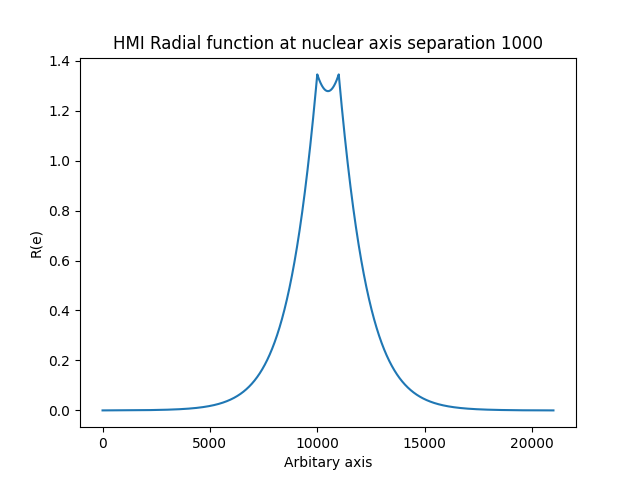
\includegraphics[scale=0.7]{"images/HMI Radial Function1000.png"}}}
		{\centering{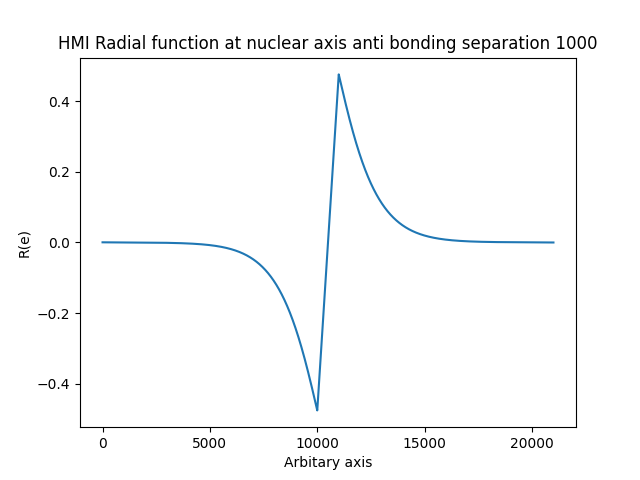
\includegraphics[scale=0.7]{"images/HMI Radial Function ab 1000.png"}}}\\
		\normalsize First for \textbf{Bonding} and second for \textbf{Anti Bonding} of HMI along inter nuclear Axis.\\
		{\centering{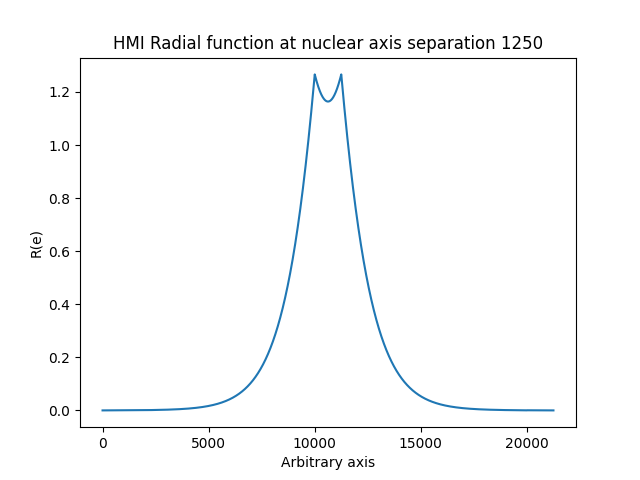
\includegraphics[scale=0.7]{"images/HMI Radial Function1250.png"}}}
		{\centering{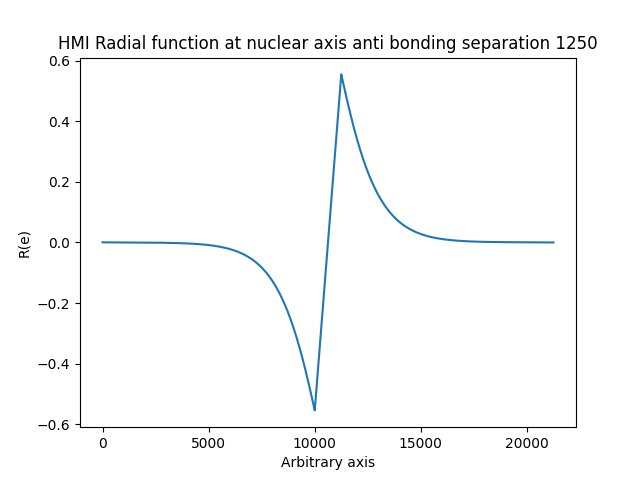
\includegraphics[scale=0.7]{"images/HMI Radial Function ab 1250.png"}}}\\
		\normalsize First for \textbf{Bonding} and second for \textbf{Anti Bonding} of HMI along inter nuclear Axis.\\
		{\centering{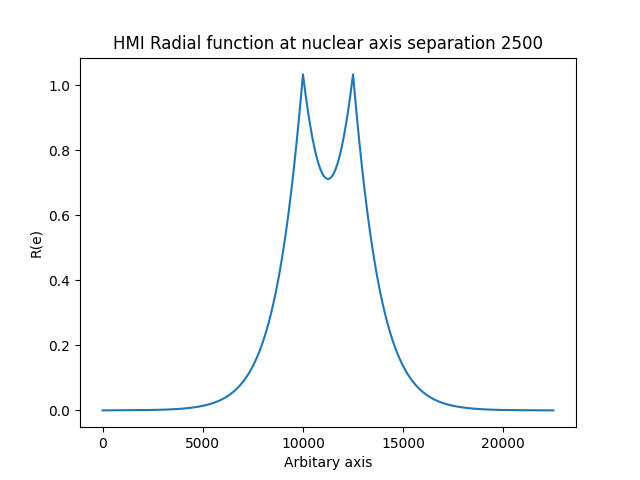
\includegraphics[scale=0.7]{"images/HMI Radial Function2500.png"}}}
		{\centering{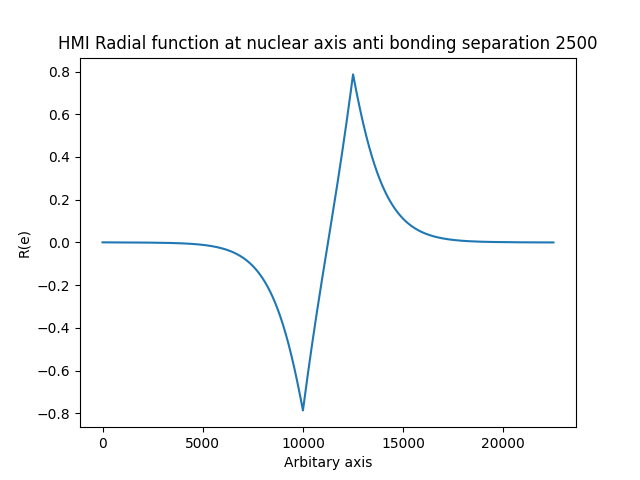
\includegraphics[scale=0.7]{"images/HMI Radial Function ab 2500.png"}}}\\
		\normalsize First for \textbf{Bonding} and second for \textbf{Anti Bonding} of HMI along inter nuclear Axis.\\
		{\centering{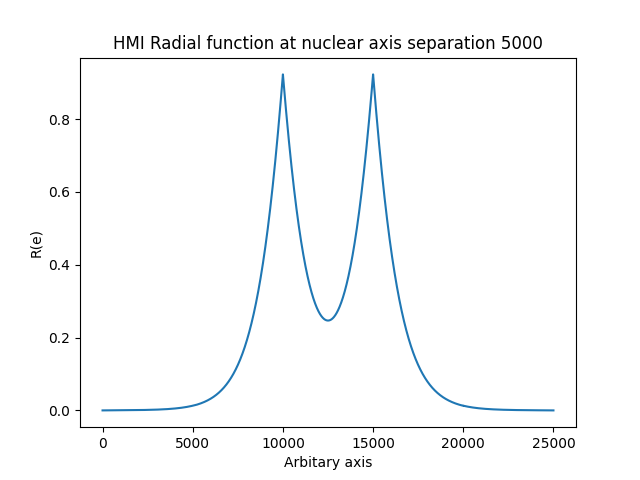
\includegraphics[scale=0.7]{"images/HMI Radial Function5000.png"}}}
		{\centering{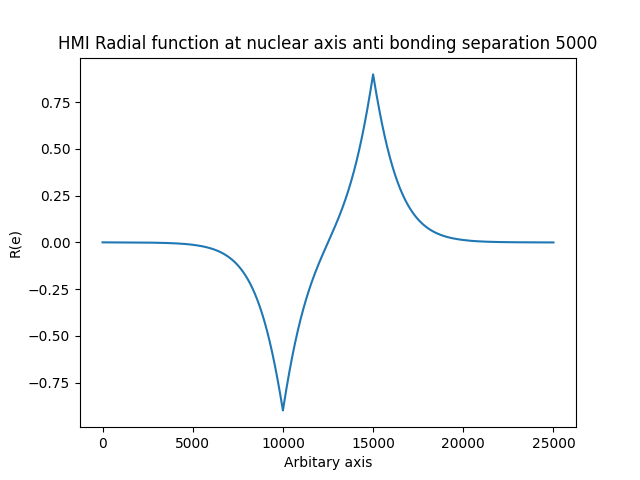
\includegraphics[scale=0.7]{"images/HMI Radial Function ab 5000.png"}}}\\
		\normalsize First for \textbf{Bonding} and second for \textbf{Anti Bonding} of HMI along inter nuclear Axis.\\
	\section{Wave Function of electron of HMI}
		\normalsize \textbf{Disclaimer:} The x-axis and y-axis are just any arbitrary axis it just gives visual representation only of inter nuclear distance. \\
		{\centering{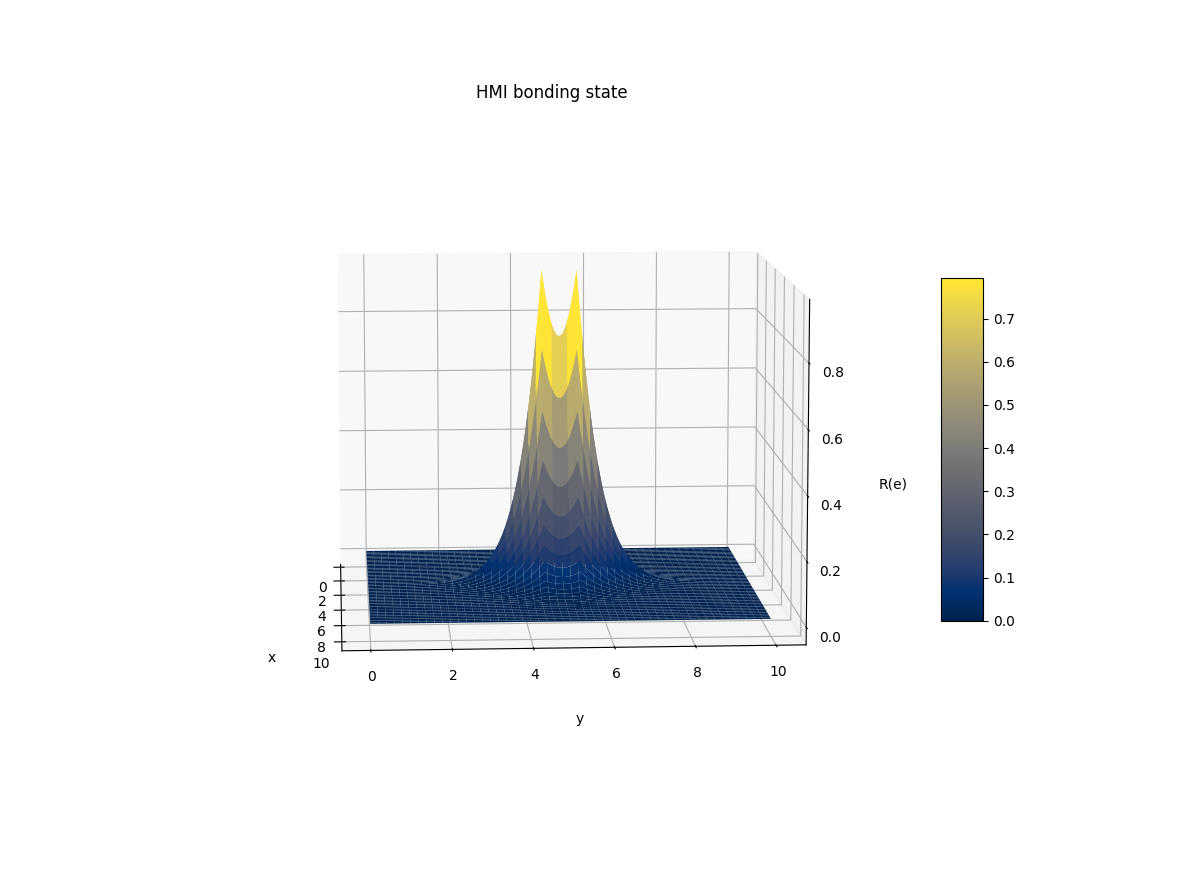
\includegraphics[scale=0.4]{"images/HMI Bonding .png"}}}\\
		{\centering{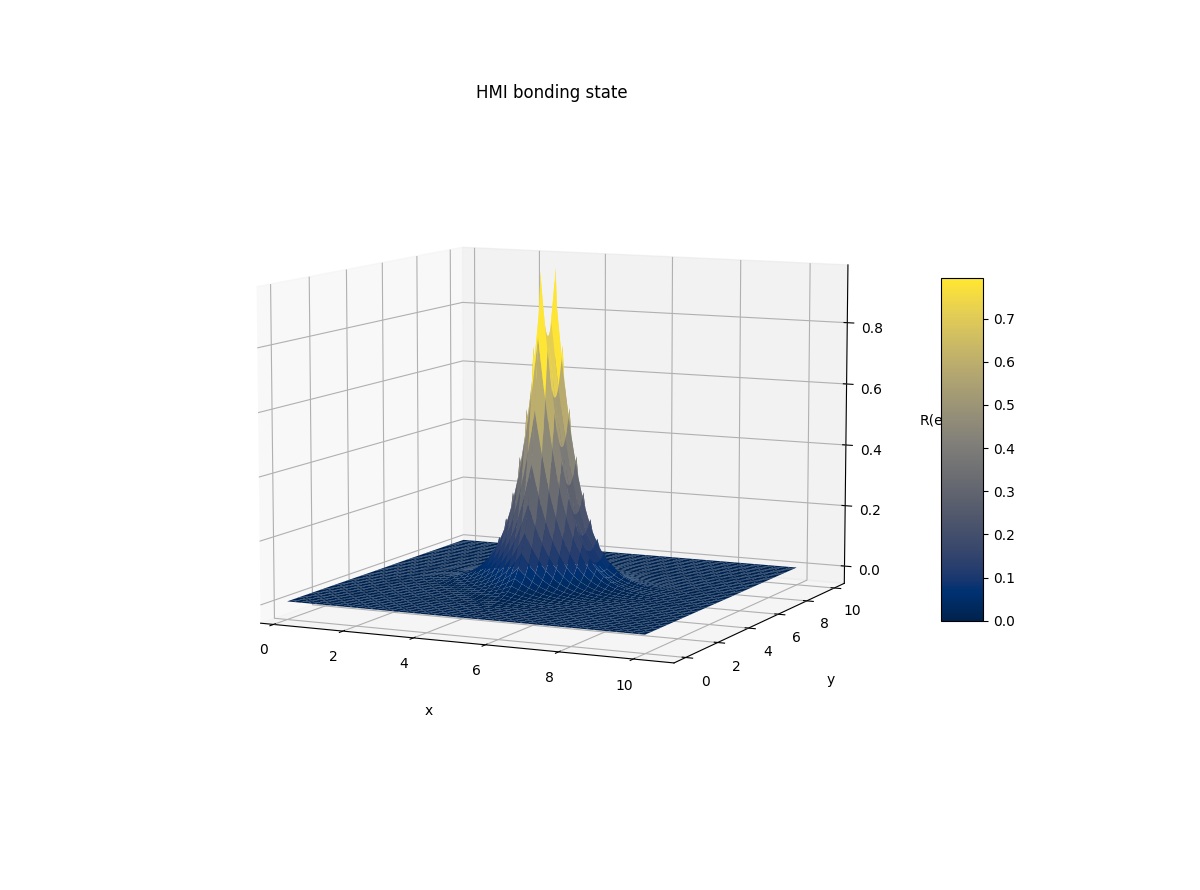
\includegraphics[scale=0.4]{"images/HMI Bonding 2.png"}}}\\
		\centering \textbf{\normalsize Bonding}\\
		\vspace{-1cm}
		{\centering{\includegraphics[scale=0.4]{"images/HMI Anti Bonding.png"}}}\\
		{\centering{\includegraphics[scale=0.6]{"images/HMI Anti Bonding 2.png"}}}\\
		\centering \textbf{\normalsize Anti Bonding}
	\section{Electron Cloud of HMI in 2D}
	    {\centering{\includegraphics[scale=0.85]{"images/electron cloud.png"}}}\\
	    \centering \textbf{\normalsize Here x and y-axis both have distance in multiple of 0.526A,and proton are at 1 and -1}\\
	    
\chapter{References}
	\begin{itemize}
		\item \normalsize \textbf{Paper: \\}\url{https://home.uni-leipzig.de/~physik/sites/mona/wp-content/uploads/sites/3/2017/04/the_hydrogen_molecular_ion_revisited.pdf}
		
		\item \normalsize \textbf{Source Code: \\}\url{https://github.com/sourabh945/Hydrogen-Molecule-Ion.git}
	\end{itemize}
\chapter{Appendix:}
	\raggedright
	\section{Scheme use for declaring the variables:}
		\begin{itemize}
			\large
			\item $\xi$ = e
			\item $\eta$ = n
			\item $\Lambda$ = \text{c\_s}
			\item $c^2$ = c2
		\end{itemize}
	\section{Source-Code}
		\subsection{Program for finding the energy eigenvalue of the HMI using Shooting Method:}
			 \lstinputlisting[language=fortran]{"Energy eigenvalue finder.f95"}
		\subsection{Program for solve for Radial and Angular wave equation, and also find the Electron Cloud for HMI:}
			\lstinputlisting[language=fortran]{"main.f95"}
		\subsection{Python Program for Operate on the files and generate the graphs for the HMI orbit:}
			\lstinputlisting[language=python]{processingfile.py}
\end{document}